a)
\begin{figure}[h]
    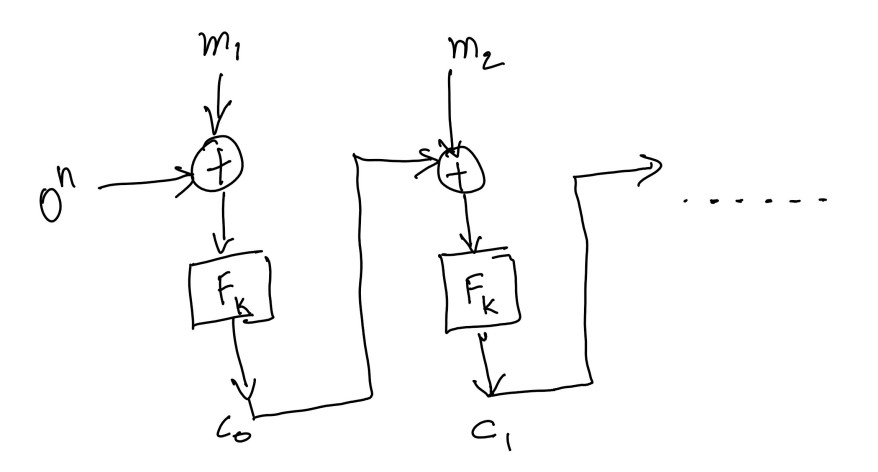
\includegraphics[width=\textwidth,height=\textheight,keepaspectratio]{7-3 IMG.jpg}
    \centering
\end{figure}


Let us consider two pair of messages and their MACs, $(m', t')$ and $(m'', t'')$

And let 
\begin{center}
    $m' = \{m_1, m_2 \}$ \\
    $m'' = \{m_1\}$ 
\end{center}

so

\begin{center}
    $c_0 = F_k(m_1)$\\
    $c_1 = F_k(m_2 \xor F_k(m_1))$
\end{center}

So as per the message MAC pair we considered 
\begin{center}
    $t' = c_1$\\
    $t''= c_0$
\end{center}

Now consider a new message $m''' = \{m_1, m_2, (m_1 \xor t')\}$. MAC for this new 
message is 
\begin{center}
    $t''' = F_k(c_1 \xor (m_1 \xor t'))$\\
\end{center}
    replace $t'$ with $c_1$\\
\begin{center}
    $t''' = F_k(c_1 \xor (m_1 \xor c_1))$ \\
    $t''' = F_k(m_1)$\\
    $t''' = c_0$
\end{center}

So now there exists a possibility to create a third message and MAC pair created
$(m''', t''')$ with a valid MAC. As this is a valid forgery, this CBC is not secure.\\



b) 
Similar to the solution in part (a),

Now if we consider message and MAC pairs as in (a), where 
\begin{center}
    $t' = \{c_0, c_1\}$\\
    $t'' = \{c_0\}$\\
\end{center}

There exists a third message and MAC pair as
\begin{center}
    $m''' = \{m_1, m_2, (m_1 \xor t')\}$\\
    $t''' = \{c_0,c_1,c_0\}$\\
\end{center}

Again this is a valid forgery! and no longer secure.